\documentclass[17pt,landscape]{foils}
\usepackage[latin1]{inputenc}
\usepackage[T1]{fontenc}
\usepackage[french]{babel}
\usepackage{amsmath,amsthm}
\usepackage{amssymb}
\usepackage{fancyhdr}
\usepackage[pdftex]{graphicx,graphics,color}
\usepackage[colorlinks]{hyperref}
\cfoot{\small{}} \pagestyle{fancy} \hypersetup{pdftitle={A mixed
linear model with change-points for the analysis multiple patients
of CGH data},
           pdfauthor={Emilie LEBARBIER},
           pdfpagemode={FullScreen}
}


\textwidth 24cm \textheight 20cm \topmargin 0cm \oddsidemargin 0cm
\evensidemargin 0cm

\newcommand{\coefbin}[2]{\left(
    \begin{array}{c} #1 \\ #2 \end{array}
  \right)}
  \newcommand{\Bcal}{\mathcal{B}}
\newcommand{\Ccal}{\mathcal{C}}
\newcommand{\Dcal}{\mathcal{D}}
\newcommand{\Ecal}{\mathcal{E}}
\newcommand{\Gcal}{\mathcal{G}}
\newcommand{\Mcal}{\mathcal{M}}
\newcommand{\Ncal}{\mathcal{N}}
\newcommand{\Pcal}{\mathcal{P}}
\newcommand{\Qcal}{\mathcal{Q}}
\newcommand{\Lcal}{\mathcal{L}}
\newcommand{\Tcal}{\mathcal{T}}
\newcommand{\Ucal}{\mathcal{U}}
\newcommand{\alphabf}{\mbox{\mathversion{bold}{$\alpha$}}}
\newcommand{\betabf}{\mbox{\mathversion{bold}{$\beta$}}}
\newcommand{\gammabf}{\mbox{\mathversion{bold}{$\gamma$}}}
\newcommand{\mubf}{\mbox{\mathversion{bold}{$\mu$}}}
\newcommand{\thetabf}{\mbox{\mathversion{bold}{$\theta$}}}
\newcommand{\Pibf}{\mbox{\mathversion{bold}{$\Pi$}}}
\newcommand{\psibf}{\mbox{\mathversion{bold}{$\psi$}}}
\newcommand{\Sigmabf}{\mbox{\mathversion{bold}{$\Sigma$}}}
\newcommand{\taubf}{\mbox{\mathversion{bold}{$\tau$}}}
\newcommand{\Ebf}{{\bf E}}
\newcommand{\Gbf}{{\bf G}}
\newcommand{\Hbf}{{\bf H}}
\newcommand{\Ibf}{{\bf I}}
\newcommand{\mbf}{{\bf m}}
\newcommand{\Obf}{{\bf 0}}
\newcommand{\Rbf}{{\bf R}}
\newcommand{\Sbf}{{\bf S}}
\newcommand{\Tbf}{{\bf T}}
\newcommand{\Ubf}{{\bf U}}
\newcommand{\Vbf}{{\bf V}}
\newcommand{\xbf}{{\bf x}}
\newcommand{\Xbf}{{\bf X}}
\newcommand{\Wbf}{{\bf W}}
\newcommand{\Ybf}{{\bf Y}}
\newcommand{\Zbf}{{\bf Z}}
\newcommand{\Esp}{{\mathbb E}}
\newcommand{\Var}{{\mathbb V}}
\newcommand{\Cov}{{\mathbb C}\mbox{ov}}
\newcommand{\Ibb}{{\mathbb I}}
\newcommand{\Rbb}{\mathbb{R}}
\renewcommand{\baselinestretch}{1.3}
\newdimen\AAdi%
\newbox\AAbo%
\newcommand{\emphase}[1]{\textblue{\sl #1}}
\def\argmax{\mathop{\mathrm{argmax}}}
\newcommand{\ec}[1]{\mathbb{E}_{\phi^{(h)}}\left\{#1 |{\Ybf} \right\}}
\newcommand{\vc}[1]{\mathbb{V}_{\phi^{(h)}}\left\{#1 |{\Ybf} \right\}}
\newcommand{\var}{\mathbb{V}}

\title{\large{A mixed linear model with breakpoints for the
analysis of multiple CGH arrays}}

\author{ E. Lebarbier, S. Robin \\
      \footnotesize {UMR INA P-G/ENGREF/INRA MIA 518, Paris, France} \\
      F. Picard \\
      \footnotesize {UMR CNRS-8071/INRA-1152/Universit\'e d'\'Evry, \'Evry, France}\\
      Eva Budinsk\`a \\
      \footnotesize {Centre of Biostatistics and Analyses, Faculty of Science and Faculty
of Medicine, Masaryk University, Brno}   }



\date{}

\begin{document}


\maketitle \MyLogo{}
\definecolor{gris}{rgb}{0.9,0.9,0.9}
\definecolor{bleufonce}{rgb}{0,0,0.5}
%\color{bleufonce} %\pagecolor{gris}
\newcommand{\textblue}[1]{\textcolor{blue}{#1}}
\newcommand{\section}[1]{\centerline{\large \textblue{#1}}}
\newcommand{\paragraph}[1]{\noindent {\textblue{#1}}}
\newcommand{\textred}[1]{\textcolor{red}{#1}}
\newcommand{\textgreen}[1]{\textcolor{green}{ #1}}

%%%%%%%%%%%%%%%%%%%%%%%%%%%%%%%%%%%%%%%%%%%%%%%%%%%%%%%%%%
%%%%%%%%%%%%%%%%%%%%%%%%%%%%%%%%%%%%%%%%%%%%%%%%%%%%%%%%%%
\newpage
\chead{\large {Multiple arrays analysis}} \foilhead[-.5in]{}

\vspace{1cm}

\paragraph{Example : comparing groups of patients}
To detect chromosomal aberrations associated with a specific
disease, we compare the profiles of healthy and disease patients, or
the profiles of group of patients with different prognosis.


\paragraph{Data.}
\begin{itemize}
\item Institut Curie (O. Delattre, Y. de Rycke)

\item Nakao et al (2004) \\

\end{itemize}


\paragraph{First approach : Common breakpoints:} all patients within the same group have their breakpoints at the
same positions.

\noindent $\Rightarrow$ That corresponds to segment a \textit
{multivariate} signal (as many dimensions as patients). \\
This can be done with a generalization of the model presented above
and with the same algorithm.

%%%%%%%%%%%%%%%%%%%%%%%%%%%%%%%%%%%%%%%%%%%%%%%%%%%%%%%%%%
\newpage
\chead{\large {Curie dataset: Chromosome 8}} \foilhead[-.5in]{}

%\vspace{1.5cm}

\begin{tabular}{ccc}
  & Good prognosis (53 patients) & Bad prognosis (81 patients) \\
  \hspace{-1cm}
  \begin{tabular}{p{2.5cm}} Number of breakpoints \end{tabular} &
  \begin{tabular}{c}
 % \begin{figure}
  %\begin{center}
  \includegraphics[scale=0.4]{CurieChromo8Gp1_K.png}
 % \end{center}
 %     \end{figure}
  \end{tabular}
  &
  \begin{tabular}{c}
  %\begin{figure}
  \includegraphics[scale=0.4]{CurieChromo8Gp2_K.png}
  %    \end{figure}
  \end{tabular} \\
  \hspace{-1cm}
  \begin{tabular}{p{2.5cm}} Position of the breakpoints \end{tabular} &
  \begin{tabular}{c}
   % \begin{figure}
  \includegraphics[scale=0.4]{CurieChromo8Gp1_T.png}
    %  \end{figure}
  \end{tabular}
  &
  \begin{tabular}{c}
   % \begin{figure}
  \includegraphics[scale=0.4]{CurieChromo8Gp2_T.png}
    %  \end{figure}
  \end{tabular}
\end{tabular}

\noindent Common breakpoints: no adapt and no relevant biologically.





%%%%%%%%%%%%%%%%%%%%%%%%%%%%%%%%%%%%%%%%%%%%%%%%%%%%%%%%%%
\newpage
\chead{\large {Mixed linear model with breakpoints}}
\foilhead[-.5in]{}


\paragraph{Proposed model.}

$\rightarrow$ We allow patient-specific segmentation.

$\rightarrow$ \emphase{Assumption:} the profiles of patients within
a same group at same position are \emphase{correlated}.


\paragraph{Model.} $Y_{g\ell t}$ denotes the observed logratio at position $t$
for patient $\ell$ within group $g$. We assume that
$$
Y_{g\ell t} = \mu_{g\ell k} + U_{gt} + E_{g\ell t} \qquad \mbox{if
position $t$ belongs to segment $I_{g\ell k}$}
$$
where
\begin{itemize}
\item $I_{g\ell k}$ is the $k$-th segment of patient
  $\ell$ from group $g$,
\item  $\mu_{g\ell k}$ is the mean signal in segment
  $I_{g\ell k}$,
\item  $U_{gt}$ is the random effect at position $t$ in
  group $g$: $\{U_{gt}\}$ independent, $U_{gt} \sim \Ncal(0,
  \sigma^2_g)$,
\item $E_{g\ell t}$ is the noise: $\{E_{g\ell t}\}$
  i.i.d. $\sim \Ncal(0, \sigma^2_0)$.
\end{itemize}

\vspace{-.5cm}

$$
\Cov(Y_{g\ell t}, Y_{g'\ell' t'}) =  \sigma^2_g \quad \mbox{ if
  \textblue{same group $g$ and same position $t$}}.
$$

%%%%%%%%%%%%%%%%%%%%%%%%%%%%%%%%%%%%%%%%%%%%%%%%%%%%%%%%%%
\newpage
\chead{\large {General model writing}} \foilhead[-.5in]{}


$$
\Ybf = \underset{\mbox{Covariates}}{\underbrace{\Xbf \thetabf}} +
\underset{\mbox{Segmentation}}{\underbrace{\Tbf \mubf}} +
\underset{\mbox{Random effects}}{\underbrace{\Zbf \Ubf}} + \Ebf
$$

\vspace{1cm}

where $G = $ number of groups, $L =$ number of patients per group,
$M =$ number of positions, $K =$ total number of segments, $N = GLM
=$ total number of data and \\
\begin{description}
\item[$\bullet \Ubf \; (GM \times 1)$] \vspace{-0.5cm} (unobserved) and $\sim \Ncal(\Obf, \Gbf)$
  (\emphase{$\Gbf$ unknown $\rightarrow$ to estimate}), \\

\item[$\bullet \Ebf \; (N \times 1)$] \vspace{-0.5cm} residual (unobserved):
  $\Ebf \sim \Ncal(\Obf, \Rbf)$ (\emphase{$\Rbf$ diagonal, unknown
    $\rightarrow$ to estimate}), \\

\item[$\bullet \Ubf$ and $\Ebf$] are independent.
\end{description}




%%%%%%%%%%%%%%%%%%%%%%%%%%%%%%%%%%%%%%%%%%%%%%%%%%%%%%%%%%
\newpage
\chead{\large {Parameters estimation}} \foilhead[-.5in]{}



\paragraph{Direct maximisation of the likelihood.}
The distribution of $\Ybf$ is
$$
\Ybf \sim \Ncal(\Xbf \thetabf + \Tbf \mubf, \Vbf), \qquad
\mbox{where
  } \Vbf = \Zbf \Gbf \Zbf' + \Rbf.
$$
Because, $\Vbf$ is not diagonal, the direct maximisation of the
observed log-likelihood $\Lcal(\Ybf)$ leads to the minimisation of a
non additive contrast in $K$.

\centerline{Dynamic programming \emphase{can not be used} to
estimate
  $\Tbf$ and $\mubf$}




\paragraph{Idea.}
$$
\Ybf -\Xbf \thetabf - \Zbf \Ubf \; | \; \Ubf \sim \Ncal(\Tbf \mubf,
\Rbf).
$$
$\Rbf$ is diagonal so the contrast to be minimized is additive in
$K$.

\centerline{\emphase{Dynamic programming can be used to estimate
    $\Tbf$ and $\mubf$}}

\paragraph{E-M strategy.} (used by Foulley (Lecture note, 2004) for mixed linear models) the
unobserved effect $\Ubf$ is predicted.




%%%%%%%%%%%%%%%%%%%%%%%%%%%%%%%%%%%%%%%%%%%%%%%%%%%%%%%%%%
\newpage
\chead{\large {E-M strategy}} \foilhead[-.5in]{}

\paragraph{Idea.} The model can be viewed as model with incomplete data
: \emphase{$U$ is hidden}.


\paragraph{Principle.}
In presence of incomplete data, the maximisation of $\Lcal(\Ybf)$ is
equivalent to the maximisation of the conditional expectation
$$
\Qcal = \Esp\left[\Lcal(\Ybf, \Ubf) \; | \; \Ybf \right] =
\underset{\mbox{$\Qcal_0$}}{\underbrace{\Esp\left[\Lcal(\Ybf| \Ubf)
\; | \; \Ybf \right]}} +
\underset{\mbox{$\Qcal_1$}}{\underbrace{\Esp\left[\Lcal(\Ubf) \; |
\; \Ybf \right]}}.
$$

Here we have
\begin{eqnarray*}
-2 \Qcal_0& = & N \log(2\pi) +\log(|\Rbf|^{-1}) +\| \Ybf-\Xbf \thetabf -\Tbf \mubf- \Zbf \Esp(\Ubf|\Ybf)\|^2_{\Rbf^{-1}}\\
              && +  \text{Tr} \left( \Rbf^{-1} \Zbf \Var(\Ubf|\Ybf) \Zbf' \right) \\
-2\Qcal_1 & = & M \log(2\pi)+ \log(|\Gbf|^{-1}) + \Esp(\Ubf|\Ybf)'
\Gbf^{-1} \Esp(\Ubf|\Ybf)+\text{Tr} \left( \Gbf^{-1} \Var(\Ubf|\Ybf)
\right) 
\end{eqnarray*}





%%%%%%%%%%%%%%%%%%%%%%%%%%%%%%%%%%%%%%%%%%%%%%%%%%%%%%%%%%
\newpage
\chead{\large {ECM algorithm (Expectation/Conditional
Maximization)}} \foilhead[-.5in]{}


\paragraph{Notation.} Denoted by $\phi=(\mubf,\thetabf,\Gbf,\Rbf,\Tbf)$ the set of parameters to be
estimated.

\vspace{1cm}

At the iteration $(h)$

\paragraph{E-step.} Calculation of $Q(\phi; \phi^{(h)})=\ec{\log
    \mathcal{L}(\Ybf,\Ubf;\phi)}$: we need the calculation of
\begin{eqnarray*}
  \widehat{\Ubf}^{(h)}=\ec{\Ubf} & = & \Gbf^{(h)} \Zbf' \Vbf^{-1} \left (\Ybf-\Xbf
\thetabf^{(h)}-\Tbf ^{(h)} \mubf^{(h)} \right ),
\end{eqnarray*}
the BLUP of the random effects $\Ubf$ and
\begin{eqnarray*}
\Wbf^{(h)} =\vc{\Ubf} & = & \Gbf^{(h)} \left [ I_N - \Zbf' \Vbf^{-1}
\Zbf \Gbf^{(h)} \right]
\end{eqnarray*}

%%%%%%%%%%%%%%%%%%%%%%%%%%%%%%%%%%%%%%%%%%%%%%%%%%%%%%%%%%
\newpage
\chead{\large {ECM algorithm (Expectation/Conditional
Maximization)}} \foilhead[-.5in]{}


\paragraph{Problem.} We need the inversion of the matrix $\Vbf$ which
is in general untractable.


\paragraph{Henderson's trick.} We solve

$$
\left[
\begin{array}{cc}
\Xbf ' \Rbf^{-1} \Xbf     &  \Xbf' \Rbf^{-1} \Zbf  \\
\Zbf' \Rbf^{-1} \Xbf   & \Zbf' \Rbf^{-1} \Zbf +\Gbf^{-1}      \\
\end{array}
\right] \left[
\begin{array}{c} \thetabf^{(h)} \\ \widehat{\Ubf}^{(h)}
\end{array}
\right] = \left[
\begin{array}{c}
\Xbf' \Rbf^{-1} \Ybf \\ \Zbf' \Rbf^{-1} \Ybf
\end{array}
\right]
$$


\paragraph{Simplification of $\widehat{\Ubf}$ and $\Wbf$.} We obtain


\begin{eqnarray*}
  \widehat{\Ubf}^{(h)} & = &  \Wbf^{(h-1)} \Zbf^{\prime} \Rbf^{(h)-1}
  \left(\Ybf-\Xbf \thetabf^{(h)}-\Tbf^{(h)}  \mubf^{(h)}\right), \\
  \Wbf^{(h)} & = &\left(\Zbf^{\prime} \Rbf^{(h)-1} \Zbf +
  \Gbf^{(h)-1} \right)^{-1}.
\end{eqnarray*}




%%%%%%%%%%%%%%%%%%%%%%%%%%%%%%%%%%%%%%%%%%%%%%%%%%%%%%%%%%
\newpage
\chead{\large {ECM algorithm (Expectation/Conditional
Maximization)}} \foilhead[-.5in]{}




\paragraph{CM-steps.} Maximization of the obtained $Q(\phi; \phi^{(h)})$. Each step focus on one parameter:

\begin{description}
\item[Estimation of $\thetabf$.] The update of $\thetabf$ is done
with the classical least-squares estimator
\begin{equation*}
  \Xbf' \Rbf^{(h)-1} \Xbf \thetabf^{(h+1)} = \Xbf' \Rbf^{(h)-1} (\Ybf
  - \Tbf^{(h)} \mubf^{(h)}- \Zbf \widehat{\Ubf}^{(h)}).
\end{equation*}

\item[Estimation of the variance $\Gbf$ and $\Rbf$.]
\begin{eqnarray*}
\Gbf^{(h+1)}&=&\arg \max_{\Gbf} Q_1 (\phi;
\thetabf^{(h+1)},\Tbf^{(h)},\mubf^{(h)}, \Gbf^{(h)},
\Rbf^{(h)}) \\
\Rbf^{(h+1)}&=&\arg \max_{\Rbf} Q_0 ( \phi; \thetabf^{(h+1)},
\Tbf^{(h)}, \mubf^{(h)}, \Gbf^{(h+1)}, \Rbf^{(h)})
\end{eqnarray*}
\item[Estimation of segmentation parameters $\Tbf \mubf$.]

\begin{eqnarray*}
\left\{ \Tbf^{(h+1)},\mubf^{(h+1)} \right\} & = & \arg
\max_{\Tbf,\mubf} Q_0 \left(\phi;
  (\thetabf^{(h+1)},\Gbf^{(h+1)},\Rbf^{(h+1)})\right),\\
&=& \arg\min_{\Tbf\mubf} \|\Ybf - \Xbf
\thetabf^{(h+1)}-{\Tbf\mubf}-\Zbf \widehat{\Ubf}^{(h)})\|^2
\end{eqnarray*}


\end{description}

%%%%%%%%%%%%%%%%%%%%%%%%%%%%%%%%%%%%%%%%%%%%%%%%%%%%%%%%%%
%%%%%%%%%%%%%%%%%%%%%%%%%%%%%%%%%%%%%%%%%%%%%%%%%%%%%%%%%%
\newpage
\chead{\large {Implementation strategy : the segmentation step}}
\foilhead[-.5in]{}

\paragraph{Optimization problem.} We have to minimize
\begin{eqnarray*}
SSR_{K}(\mubf, \Tbf) &=& \| \Ybf-\Xbf \thetabf^{(h+1)} -\Tbf \mubf-
\Zbf \widehat{\Ubf}^{(h)}\|^2\\
& = &  \sum_{l=1}^{L} \sum_{k=1}^{K_l} SSR^l_k(\mubf_l,\Tbf_l)
\end{eqnarray*}
under the constraint $\sum_l K_l=K$. \\

$\rightarrow$ This minimization is achieved thanks to dynamic
programming since the contrast to be minimized is additive in $K$.

$\rightarrow$ However this is computationally heavy.


%%%%%%%%%%%%%%%%%%%%%%%%%%%%%%%%%%%%%%%%%%%%%%%%%%%%%%%%%%
%%%%%%%%%%%%%%%%%%%%%%%%%%%%%%%%%%%%%%%%%%%%%%%%%%%%%%%%%%
\newpage
\chead{\large {Implementation strategy : the segmentation step}}
\foilhead[-.5in]{}


\paragraph{Proposed strategy.} We propose to use a two stage dynamic programming
algorithm:
\begin{description}
\item[Stage-1] Each patient $l$ is segmented into $k=1,\ldots,K_l$
segments. This step is based on the fact that
\begin{eqnarray*}
\forall k \in [1:K_l], & \\
SSR_{k}^l(]t_{1}^l,M]) & = \min_{h}
\left\{SSR_{k-1}^l(]t_{1}^l,h])+SSR_{1}^l(]h,M]) \right\}.
\end{eqnarray*}
Denoted by $J^l$ the best segmentation of the patient $l$ into $k$
segments. \\

\item[Stage-2] This step is based on the fact that
\begin{eqnarray*}
\forall l \in [1:L], &\\
SSR_{K}(J^1,\hdots,J^l) &= \min_{k}
\left\{SSR_{k}(J^1,\hdots,J^{l-1})+SSR_{K-k}^l(J^l) \right\}.
\end{eqnarray*}

\end{description}

%\paragraph{Complexity.} Assuming that $K=M k $ with $k \lambda \ll n$ It is reduced from $\mathcal{O}(N^2 K)$ to $\mathcal{O}(K M^2+K^2
%M)$.

%%%%%%%%%%%%%%%%%%%%%%%%%%%%%%%%%%%%%%%%%%%%%%%%%%%%%%%%%%
%%%%%%%%%%%%%%%%%%%%%%%%%%%%%%%%%%%%%%%%%%%%%%%%%%%%%%%%%%
\newpage
\chead{\large {Implementation strategy : the ECM algorithm}}
\foilhead[-.5in]{}


\paragraph{'Regular' ECM.} During the CM-steps, the circular estimation of all the parameters $\sigma^2_g, \sigma^2_0,
\thetabf$ and $\Tbf\mubf$ given $\widehat{\Ubf}$ and $\Wbf$ until
convergence, but it would requires
\emphase{numerous dynamic programming steps} at each M step.\\ \\

\paragraph{Proposed strategy.} To perform few dynamic programming
steps, we iterate the E step and the circular estimation of
$\sigma^2_g, \sigma^2_0$ and $\thetabf$ until convergence, before
updating $\widehat{\Tbf\mubf}$.\\ \\

\paragraph{Numerical comparison.} The two algorithms give the
\emphase{same estimates}, but the proposed strategy is the
\emphase{most efficient} in terms of computational time.

%%%%%%%%%%%%%%%%%%%%%%%%%%%%%%%%%%%%%%%%%%%%%%%%%%%%%%%%%%
%%%%%%%%%%%%%%%%%%%%%%%%%%%%%%%%%%%%%%%%%%%%%%%%%%%%%%%%%%
\newpage
\chead{\large {Selection of the number of segments $K$}}
\foilhead[-.5in]{}

\paragraph{Model selection.}
\begin{equation*}
\widehat{K}=\argmax_{K} \left \{ \Lcal(\Ybf; \widehat{\phi}) -pen(K)
\right \}
\end{equation*}

\paragraph{Penalty.}

\begin{equation*}
pen(K)=\alpha \left \{ \text{Number of parameters of model of
K-dimensional} \right \} \left( 2 \log{N/K}+5 \right )
\end{equation*}


\paragraph{Calibration of $\alpha$} by adaptative method.

%%%%%%%%%%%%%%%%%%%%%%%%%%%%%%%%%%%%%%%%%%%%%%%%%%%%%%%%%%
%%%%%%%%%%%%%%%%%%%%%%%%%%%%%%%%%%%%%%%%%%%%%%%%%%%%%%%%%%
\newpage
\chead{\large {Application on Nakao dataset - chromosome 20}}
\foilhead[-.5in]{}

\paragraph{Data.} A cohort of $121$ colorectal cancer patients. This
cohort is divided into 4 clinical groups with respective size
$$
L_1=11 \ , \ L_2=37 \ , \ L_3=35 \ \text{and} \ \ L_4=38
$$

\paragraph{Model.}
$$
Y_{g\ell t} = \mu_{g\ell k} + U_{gt} + E_{g\ell t} \qquad \mbox{if
position $t$ belongs to segment $I_{g\ell k}$}
$$
where $\{E_{g\ell t}\} \sim \mathcal{N}(0,\sigma^2_0)$.

\paragraph{Variance structure for $\Ubf$.} We can consider several
cases:
\begin{itemize}
\item $\Var(U_{gt})= \sigma^2,$
\item $\Var(U_{gt})= \sigma^2_g,$
\item $\Var(U_{gt})= \sigma^2_{gt}.$ \\
\end{itemize}


\paragraph{First result.} We obtain very similar results for these three structures.

%%%%%%%%%%%%%%%%%%%%%%%%%%%%%%%%%%%%%%%%%%%%%%%%%%%%%%%%%%
\newpage
\chead{\large {Number of breakpoints - $\Var(U_{gt})= \sigma^2_g$ -
$\widehat{K}=240$}} \foilhead[-.5in]{}


\vspace{0.2cm}


\begin{center}
\begin{tabular}{cc}
   Stage 1 (11 patients) & Stage 2 (37 patients) \\
  \hspace{-1cm}
   \begin{tabular}{c}
  \includegraphics[scale=0.6]{hist_ruptures_nakao20_group_Kh=360_group1.png}
  \end{tabular}  &
  \begin{tabular}{c}
  \includegraphics[scale=0.6]{hist_ruptures_nakao20_group_Kh=360_group2.png}
  \end{tabular} \\
  Stage 3 (35 patients) & Stage 4 (38 patients) \\
  \hspace{-1cm}
  \begin{tabular}{c}
  \includegraphics[scale=0.6]{hist_ruptures_nakao20_group_Kh=360_group3.png}
  \end{tabular}  &
  \begin{tabular}{c}
  \includegraphics[scale=0.6]{hist_ruptures_nakao20_group_Kh=360_group4.png}
  \end{tabular}
\end{tabular}
\end{center}


%%%%%%%%%%%%%%%%%%%%%%%%%%%%%%%%%%%%%%%%%%%%%%%%%%%%%%%%%%
\newpage
\chead{\large {What is the role of the random effect?}
\emphase{Group 1} ($\widehat{K}_U=240$ and $\widehat{K}_{WU}=230$)}
\foilhead[-.5in]{}

\vspace{-0.5 cm}

\begin{tabular}{c}
  \emphase{Position of the breakpoints without (red) and with (black) the random effect}\\
  \begin{tabular}{c}
  \includegraphics[scale=1.1]{Group1_rupt.png}
  \end{tabular}\\
   \emphase{Estimation of the random effect }  \\
  \begin{tabular}{c}
  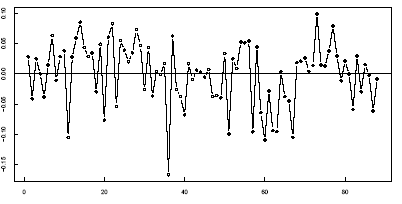
\includegraphics[scale=1.1]{Group1_U.png}
  \end{tabular}
\end{tabular}

%%%%%%%%%%%%%%%%%%%%%%%%%%%%%%%%%%%%%%%%%%%%%%%%%%%%%%%%%%
\newpage
\chead{\large {\emphase{Group 1} : the two profiles with these
changes}} \foilhead[-.5in]{}

\vspace{-.5cm}

\noindent Legend: red$=$without $U$ and black$=$ with $U$.



\begin{figure}
\begin{center}
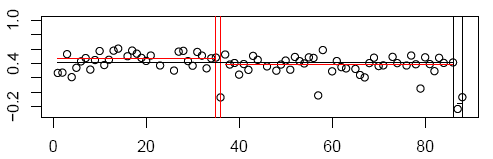
\includegraphics[scale=1]{Exemple_profile6_groupe1.png}
\end{center}
\end{figure}

\begin{figure}
\begin{center}
\includegraphics[scale=1]{Exemple_profile7_groupe1.png}
\end{center}
\end{figure}

%%%%%%%%%%%%%%%%%%%%%%%%%%%%%%%%%%%%%%%%%%%%%%%%%%%%%%%%%%
\newpage
\chead{\large { \emphase{Group 3} (results similar to groups 2 and
4) }} \foilhead[-.5in]{}

\vspace{-0.5 cm}

\begin{tabular}{c}
  \emphase{Position of the breakpoints without (red) and with (black) the random effect}\\
  \begin{tabular}{c}
  \includegraphics[scale=1.1]{Group3_rupt.png}
  \end{tabular}\\
   \emphase{Estimation of the random effect }  \\
  \begin{tabular}{c}
  \includegraphics[scale=1.1]{Group3_U.png}
  \end{tabular}
\end{tabular}


%%%%%%%%%%%%%%%%%%%%%%%%%%%%%%%%%%%%%%%%%%%%%%%%%%%%%%%%%%
\newpage
\chead{\large {\emphase{Group 3} : two profiles with these changes}}
\foilhead[-.5in]{}

\vspace{-.5cm}

\noindent Legend: red$=$without $U$ and black$=$ with $U$.



\begin{figure}
\begin{center}
\includegraphics[scale=1.1]{Exemple_profiles7_24_groupe3.png}
\end{center}
\end{figure}


%%%%%%%%%%%%%%%%%%%%%%%%%%%%%%%%%%%%%%%%%%%%%%%%%%%%%%%%%%
\newpage
\chead{\large {Conclusion and perspectives}} \foilhead[-.5in]{}



\paragraph{Estimated variances.}
\begin{equation*}
(\widehat{\sigma}_g^2)_g=(0.0031 0.0027 0.0036 0.0033)
\end{equation*}
$\rightarrow$ The estimated variances are similar. \\

\paragraph{Random effect.}
\begin{itemize}
\item could help to detect particular point (as bad spot).

\item do not reveal biological information. \\
\end{itemize}

\paragraph{Other application fields}
\begin{itemize}
\item Climatic data. Breakpoint detection of the evolution of the
temperature of several cities in France.
\item Botanic data. Growth phase detection of trees.
\end{itemize}

\end{document}
